%%%%%%%%%%%%%%%%%%%%%%%%%%%%%%%%%%%%%%%%%%%%%%%%%%%%%%%%%%%%%%%%%%%%%%%%%%%%%
% Chapter 1: Introducción 
%%%%%%%%%%%%%%%%%%%%%%%%%%%%%%%%%%%%%%%%%%%%%%%%%%%%%%%%%%%%%%%%%%%%%%%%%%%%%%%
El objectivo de este proyecto es desarrollar una aplicación para la gestión de un grupo
de Scout. La aplicación deberá gestionar a los chicos asociados al grupo y mantener su 
información personal, incluyendo familiares, datos bancarios y medicos. 

La tecnologia principal usada se basa en aplicaciones web con un entorno de desarrollo de alto
nivel, en nuestro caso con el Framework de Django, y tambien con implantación en la nube, gracias a 
Google App Engine.
%---------------------------------------------------------------------------------
\section{Antecedentes y estado actual del tema}
\label{1:sec:1}
El Escultismo es un movimiento educativo fundado en el año 1907 por Baden Powell en Inglaterra
e instalado en España en 1912. Su musión es dejar este mundo mejor de como lo encontramos,
una misión que es posible gracias a una gran labor diaria y educativa que realizan de manera
voluntaria jóvenes de todo el mundo.

Hoy en día se pueden encontrar páginas web de organizaciones de grupos Scout,  pero la mayoria
son simlemente para uso informativo y darse a conocer, como es el caso del grupo Aguere 70, que carece de
una aplicación para la gestión de los propios socuts con sus tareas, que es en lo que se ennfocó este proyecto. Existe
una implementación, ya desactualizada, basada en tecnología PHP para las funciones básicas en la gestión de grupos
Scout: GNU Scout [1]. Esta implementación aunque no fue usada, sirvio para darnos una idea general
de como enfocar nuestra aplicación.

De modo que creamos una aplicación en la nube utilizando una versión de Django adaptada a Google 
App Engine, un servicio de alojamiento web que permite desarrollar aplicaciones online sin 
necesidad de administrar o mantener servidores dedicados. De esta forma, los usuarios podrán utilizarla lo antes posible, evitando 
tareas de gestión y administración de sistemas.


%---------------------------------------------------------------------------------
\section{Caracteristicas de la Aplicación}
\label{1:sec:2}
Resumen de los principales recursos utilizados en el desarrollo del proyecto.:
\begin{itemize}
  \item Framework Django-nonrel
  \item Despliegue en Google App Engine
  \item Google APIs (Google+ y Google Drive)
  \item GitHub
  \item jQuery
  \item JavaScript
  \item Bootstrap CSS
  
\end{itemize}
En los próximos capítulos se profundizará en la descripción de las herramientas empleadas en el proyecto.

%---------------------------------------------------------------------------------
\section{Actividades}
\label{1:sec:3}
El desarrollo del proyecto se organizó de las siguientes tareas:


\begin{tabular}{|p{25mm}|p{80mm}|} \hline 
\textbf{Tarea } & \textbf{Actividad} \\ \hline
Tarea1 &
Analisis de la aplicación GNU Scout [1] y el modelo de datos utilizado.
\\
\hline

Tarea 2 &
Entrevistas con los responsables de un grupo Scout para analizar las funcionalidades ya
previstas según [1] y añadir/eliminar/modificar aquellas de interés.
\\
\hline

Tarea 3 &
Montar un repositorio GIT \cite{URL:GitHub} para alojar los codigos del proyecto. Definir la
estrategia de branching.
\\
\hline

Tarea 4 &
Definir u proyecto en Pivotal tracker[3] para el seguimiento del proyecto. Esta herramienta
facilita el desarrollo siguiento metodologías ágiles.
\\
\hline

Tarea 5 & 
Desarrollo de un proyecto piloto, realizar la implantación en GAE[2] comprobando el 
funcionamiento básico de esta plataforma.
\\
\hline

Tarea 6 &
Entrevistas de seguimiento. 2º reunión con los responsables del grupo Scout para
mostrar el piloto de la aplicación, refinar diseños,etc
\\
\hline

Tarea 7 &
Desarrollo de la aplicación: implementar las funcionalidades requeridas (posibles
entrevistas a lo largo del proceso para comprobar si la implementación cumple los requisitos
del cliente: se realizarán por lo menos 4 iteraciones completas: análisis, desarrollo, test, implantación)
\\
\hline

Tarea 8 &
Puesta en producción (fase beta), formación de usuario y gestión de errores.
\\
\hline

\end{tabular}


%---------------------------------------------------------------------------------
\section{Período de Desarrollo del Proyecto}
\label{1:sec:4}

El período de elaboración del proyecto abarca desde el 11 de septiembre de 2012 cuando se presentaron las ofertas de los proyectos, 
hasta mediados de junio de 2013 que es cuando corresponden las respectivas defensas orales, pero lo que es la elaboración en sí de la aplicación del proyecto
abarcó del 30 de Enero de 2013 hasta primeros de Junio incluyendo los retoques finales y puesta a punto de la aplicación.
%------------------------------------------------------------------------------
\begin{figure}[!th]
\begin{center}
\includegraphics[width=0.5\textwidth]{images/arbolbinario.eps}
\caption{Ejemplo}
\label{fig:ArbolBinario}
\end{center}
\end{figure}
%------------------------------------------------------------------------------

